\chapter{Approach}
\label{ch:approach}
After implementing query expansion in the project report,
the challenge was to implement query expansion directly into the search engine.
As the Elasticsearch source code is poorly documented,
the choice was to implement query expansion with Lucene and then finally port it into Elasticsearch.
After implementing query expansion using Lucene,
Elasticsearch's documentation was inspected to learn how to make the implementation scalable.
It was discovered that Elasticsearch has a plugin API which can be used to extend Elasticsearch's functionality.

This chapter gives an overview of the query expansion algorithm before the implementation with Lucene and Elasticsearch is explained.

\section{Implementation}
\label{sec:implementation}
Two different platforms were used during the implementation.
The initial implementation used Lucene as the search engine.

\subsection{Algorithm}
\label{sec:algorithm}
The algorithm used for query expansion is equal on both platforms,
but they have some platform specific differences which are explained in their respective subsections.
The algorithm is available as pseudocode in appendix \ref{ap:pseudocode}.

The algorithm starts by sending a term search to the search engine.
The result from the initial search is often referred to as top-k documents,
where k stands from the number of documents in the results.
The photos from the result are then looped through to extract all the terms.
Each term is stored in a hash map for fast retrieval.
On every iteration the term is checked against the hash map.
If the term does not exists,
the term is added to the hash map.
The key is the hash map itself,
and the value is an object which stores information about the total number of times the term occurs in the whole collection,
the total number of terms in total in the collection and the number of times the term is present in the top-k documents.
In the opposite case where the term already exists, the term counter for the current term is incremented.
The counter for the number of times the term appears in the top-k documents are incremented by one.

After looping through the photos the information about how many terms there are in the whole collection is retrieved from the search engine.
Now all the information required to calculate the KL-score is available.
All the keys in the hash map are now iterated through to retrieve every single term.
In every iteration the equation \ref{eq:kl-distribution-q} is used to calculate the KL-score.
An array is used to store objects which holds information about which term it is and the corresponding KL-score.
Subsequently, the array is sorted from high to low according to their KL-score.

Next the expanded search terms need to be generated.
A new string array is created to hold the new search terms.
First the old search terms are added to the array,
then the new expanded terms are added to the array.
In this implementation a maximum of ten terms may be added to the term search.

Lastly, the expanded terms are used in a new term search.
The search engine is queried for the terms,
and the result from the search is returned directly to the client without any modifications.

\subsubsection{Algorithm Complexity}
An important aspect of every algorithm is to analyze its complexity.
The algorithm explained in \ref{sec:algorithm} has two different inputs we have to consider.
Firstly, the number of terms in top-k documents, and secondly, the number of unique terms.
This analysis only examine the algorithm itself, and does not account for the time it takes to retrieve data from the search engine.

The algorithm contains a total of three loops and one sorting algorithm.
Initially, all the tags are iterated through,
which means the size is equal to the number of tags in the top-k documents.
The second loop is of the same size as the number of unique terms.
This number has a best case of only one unique tag and a worst case of T unique terms.
Lastly, all the unique tags are sorted using a function inside the Java util library called \texttt{Arrays.sort()}.
\texttt{Arrays.sort()} uses an algorithm called merge sort,
which has a worst case of $O(n\log{}n)$.

Combining all the loops described above, the algorithm complexity  given in equation \ref{eq:algorithm-complexity}.
$T$ is the number of tags, and $U$ is the number of unique terms.

\begin{cequation}[H]
	\begin{equation}
		\mathbf{ f(T, U) } = \mathcal{O}( T + U + U\log{}U ) \\
	\end{equation}
  \caption{Algorithm complexity for the algorithm explained in subsection \ref{sec:algorithm}.}
  \label{eq:algorithm-complexity}
\end{cequation}

%\subsubsection{Algorithm Improvements}%

%From the complexity analysis one improvement becomes apparent.
%Combinding the step which counts the KL-score of each tag may be combined with the sort operation.
%However,

%Even though it is possible to improve the number of iterations in the algorithm,
%the search against the search engine have a greater impact on the response time.


%\begin{cequation}[H]
%	\begin{equation}
%		\mathbf{f(T, U)} = T + U + U\log{}U \\
%	\end{equation}
%  \caption{Algorithm complexity for the an improved version of the algorithm described in subsection \ref{sec:algorithm}.}
%  \label{eq:algorithm-improved}
%\end{cequation}

\subsection{Lucene Architecture}
The Lucene implementation were done using version 6.4.0 of Lucene \cite{lucene-documentation}.

Most search engines strives to hold the data in memory.
To achieve the performance desired by Lucene the whole index is kept in memory.

The tag field is stored with information about document frequency for each term.
The document frequency is required to calculate the KL score for each term.

Minimal Java optimizations


Even though the Lucen implementation delivered promising results, Lucene in itself is not scalable.
As one of the research questions

\texttt{IndexOptions.DOCS\_AND\_FREQS}

\subsubsection{Lucene Notes}
- Discuss java methods to retrieve term frequency from the inverted index

\subsubsection{Indexing}
Lucene have multiple data types which may be stored,
but the types used in this implementation were \texttt{StringField}, \texttt{LongPoint} and \texttt{TextField}.
All the photo tags were indexed using the \texttt{TextField}.
The two fields \texttt{TextField} and \texttt{StringField} are quite similar,
but have some important differences.
Listing \ref{lst:lucene-string-field} displays the \texttt{StringField} configuration code from Lucene's Github repository\footnote{\url{https://github.com/apache/lucene-solr/blob/master/lucene/core/src/java/org/apache/lucene/document/StringField.java}}.
The first function \texttt{setIndexOptions(IndexOptions.DOCS)},
configures the inverted index to only store which documents contains the term.
Term frequencies and vector are not stored with this option.
\texttt{setStored(true)} tells the Lucene index to store the original value.
Lastly, the function \texttt{setTokenized(false)} informs Lucene to store the string value as a single token.

\begin{lstlisting}[language=java, caption={Lucene's \texttt{StringField} index configuration.}, label={lst:lucene-string-field}]
  setStored(true);
  setTokenized(false);
  setIndexOptions(IndexOptions.DOCS);
\end{lstlisting}

Listing \ref{lst:lucene-text-field} shows the \texttt{TextField} configuration code from Lucene's Github repository\footnote{\url{https://github.com/apache/lucene-solr/blob/master/lucene/core/src/java/org/apache/lucene/document/StringField.java}}.
The difference between the \texttt{StringField} and the \texttt{TextField} code are line two and three.
\texttt{setTokenized(true)} tells the Lucene analyzer emit a token for each word in the given string.
Most important is line three which tells Lucene to store data about which documents contains a given term,
a given terms frequncy in each document and the terms position in the original text.
Calculating the KL-score of a term requires the terms total frequency across all documents.

\begin{lstlisting}[language=java, caption={Lucene's \texttt{TextField} index configuration.}, label={lst:lucene-text-field}]
    setStored(true);
    setTokenized(true);
    setIndexOptions(IndexOptions.DOCS_AND_FREQS_AND_POSITIONS);
\end{lstlisting}

\subsubsection{Query Expanded Search}
Figure shows a sequence diagram for the Lucene implementation.
As the sequence diagram shows, the java program first recieves the query.
The query is then sent to the Lucene index as a multi term query.
Lucene then returns the top-k documents from the index.



\begin{figure}[h!]
  \centering \includegraphics[width=0.9\linewidth]{img/sequence-diagram-lucene.png}
  \caption{Sequence diagram for the Lucene implementation.}
  \label{fig:sequence-diagram-lucene}
\end{figure}

\subsection{Elasticsearch Implementation}
To achieve scalability across multiple machines,
the second implementation of query expansion was done using Elasticsearch.
The initial thought was to implement query expansion directly into Elasticsearch's core.
However, during the research phase it was discovered that Elasticsearch has a plugin API.

The query expansion plugin for Elasticsearch is almost identical to the implementation described in subsection \ref{sec:algorithm} and in subsection \ref{sec:lucene}.
Thus, this subsection will only describe the differences.
The differences is mostly how the documents are indexed and how the queries are structured.

Figure \ref{fig:sequence-diagram-elasticsearch} displays the sequence diagram for the implemented Elasticsearch plugin.
First the query arrives the coordination node in the Elasticsearch cluster.
The query is parsed and distributed to all the relevant shards.
Each uses the plugin to calculate their local top-k documents.
Metadata of each shard is returned to the coordination node,
which again merges the results and calculates the global top-k documents.
Lastly,
the actual documents are retrieved from all the shards and the final result are returned.

\begin{figure}[h!]
  \centering 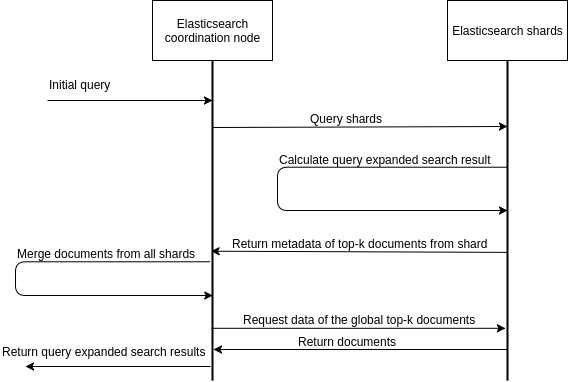
\includegraphics[width=1\linewidth]{img/sequence-diagram-elasticsearch.png}
  \caption{Sequence diagram for the Elasticsearch implementation.}
  \label{fig:sequence-diagram-elasticsearch}
\end{figure}

\subsubsection{Elasticsearch Plugin API}
\label{sec:elasticsearch-plugin-api}
Elasticsearch has it's own plugin API\footnote{\url{https://www.elastic.co/guide/en/elasticsearch/plugins/5.2/index.html}}.
This plugin API can be used to extend Elasticsearch's index and query capabilities.
The implementation described in this master thesis creates a plugin which extends the REST API with query expansion.
When a plugin is installed, the installation are done on all the nodes.
The plugin API has two main catogories: core plugins and community contributed plugins.
Core plugins are plugins which are a part of the Elasticsearch project.
These plugins are develop by the Elastic team.
Community contributed plugins, are plugins outside the Elasticsearch project.
These plugins are developed by the community.
When a plugin is installed,
the installation are distributed to all the nodes.
As the installation is distributed,
all the nodes are able to act as a coordination node,
which also makes the plugin API scalable.
The plugin implementation described in this thesis belongs to the community contributed plugins.

Accessing the extended REST API is done sending a POST request to the URL \url{http://localhost:9200/_expansion}.
This URL assumes that the server is running locally and that Elasticsearch's default port 9200 is used.
\texttt{/\_expansion} is the new REST API extension.
To send a query, the POST request need to have a body as shown in listing \ref{lst:rest-api-extension}.
The body consists of a json object with one key value pair.
The key is \texttt{search\_query} and the key is the desired query string.
Query strings with containing multiple terms are divided into separate terms.
The terms are extracted by spliting the query string on the character "space".

\begin{lstlisting}[language=json, caption={The POST request body for the implemented query expansion.}, label={lst:rest-api-extension}]
{
  "search_query": "search terms"
}
\end{lstlisting}

\subsubsection{Indexing}
Many storage solutions requires the stored data types to be defined before inserting data.
Elasticsearch have support to both predefined data types and data types determined at index time.
Data types determined while indexing is called dynamic mapping, and predefined data types are called static mapping.
Dynamic mapping are useful when prototyping and developing.
However, dynamic mapping may assign wrong types to a field.
For instance one might have a geo location point.
A geo location point will most likely be sent to Elasticsearch as two floats, latitude and longitude.
It is fine to store the values as floats, but Elasticsearch have separate data type for latitude and longitude called Geo-point.

With static mapping on the other hand, every mapping type are defined before indexing.
Static mapping ensures that each field is assigned the correct mapping.
The mapping used in this master thesis is available in appendix \ref{ap:elasticsearch-mapping}.

\subsubsection{Searching}
All the searches in the Elasticsearch implementation is similar to the searches described in the Lucene implementation,
but there are a few important differences.
The query expansion algorithm requires three different types of search:
single term query, multiple term query and field stats query.

The first step of the algorithm is to retrieve the top-k documents.
In elasticsearch this is done as a multiple term query,
and the implemented Java code is available in appendix \ref{ap:multiple-term-query}.

Retrieving the number of times a term appears in the collection may be done through Elasticsearch's count API.
However, this API is not available through the Java client library.
Instead this information may be fetched using a normal single term query.
Metadata from the search result contains the needed information.
Listing \ref{ap:elasticsearch-metadata} displays an example on how the returned result may look.
The array \texttt{hits} is intentionally left out to keep the example short,
as the array contains the search result itself.
The search result consists of information about how long the search took, how many shards searched, the total number of hits,
the maximum returned document score and the search result itself.
In listing \ref{ap:elasticsearch-metadata} there is a field called \texttt{total},
which indicates the total number of hits the term query produced.

Lastly, the query expansion also requires to know the total number of terms in the collection.
This information can be retrieved using Elasticsearch's field stats API.
The API exposes native Lucene index function,
for retrieving metadata from the inverted index.

\begin{lstlisting}[language={json}, caption={Example of the metadata returned by Elasticsearch.}, label={ap:elasticsearch-metadata}]
{
  "took": 3,
  "timed_out": false,
  "_shards": {
    "total": 5,
    "successful": 5,
    "failed": 0
  },
  "hits": {
    "total": 2912,
    "max_score": 9.73782,
    "hits": [
      ...
    ]
  }
}
\end{lstlisting}

\subsubsection{Architecture}
The architecture of the implementation can be seen in figure \ref{fig:elasticsearch-architecture}.
As described earlier,
the query first arrives a coordination node before it is parsed and sent to the data nodes in the cluster.
Node 2 is enlagred to display what this master thesis have implemented.
In figure \ref{fig:elasticsearch-architecture} the node contains a plugin called "Query Expansion,"
together with data called shard 1 and replica 1.
When a request of a certtain format arrives the plugin handles the request.
The format is explained in section \ref{sec:elasticsearch-plugin-api}.
After the plugin have calculated the top-k documents the result is returned back to the coordination node,
and later returned to the client.

\begin{figure}[h!]
  \centering 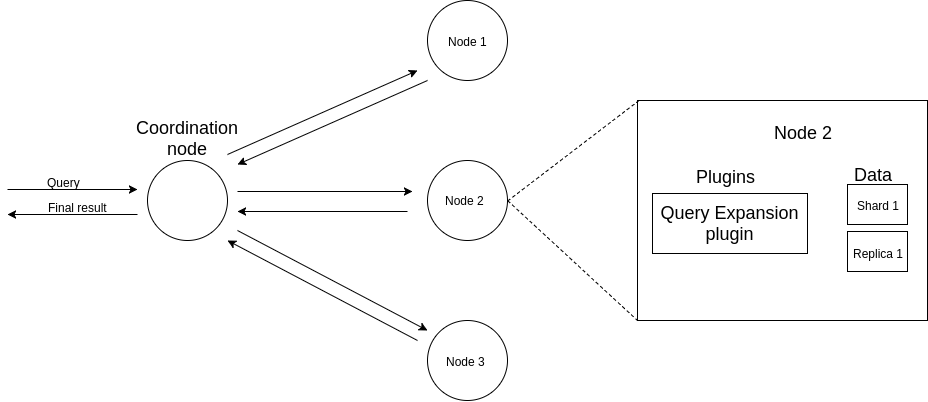
\includegraphics[width=1\linewidth]{img/elasticsearch-architecture.png}
  \caption{Architecture for the implemented Elasticsearch plugin. The figure is an example of a cluster setup with a view inside one of the node in the cluster.}
  \label{fig:elasticsearch-architecture}
\end{figure}


